
\documentclass[12pt,a4paper]{article}

\usepackage[T2A]{fontenc}
\usepackage[utf8]{inputenc}
\usepackage[russian]{babel}
\usepackage{amsmath}
\usepackage{geometry}
\usepackage{graphicx}
\usepackage{float}
\usepackage{longtable}
\usepackage{array}
\usepackage{booktabs}

\geometry{margin=2.5cm}

\title{Отчёт по задаче случайного поиска}
\author{}
\date{апрель 2026}

\begin{document}

\maketitle

\section*{Постановка задачи}

Требовалось реализовать методы случайного поиска для четырёх функций:
\begin{enumerate}
    \item $J_1(x,y)=x^2+y^2$;
    \item $J_2(x,y)=x^2/4+y^2/9$;
    \item $J_3(x,y)=70(x-1)^2+(y-1)^2+1$;
    \item $J_4(x,y)=(x-8)^2+(y-1)^2+70(y+(x-8)^2-1)^2+1$.
\end{enumerate}

Для каждой функции были реализованы три алгоритма:
\begin{enumerate}
    \item алгоритм с возвратом при неудачном шаге;
    \item алгоритм наилучшей пробы;
    \item алгоритм статистического градиента.
\end{enumerate}

\section*{Принятые допущения}

Так как в исходной постановке не были заданы конкретные параметры шага и количества проб, использовались разумные настройки:
\begin{itemize}
    \item в методах случайного поиска шаг уменьшался после серии неудачных итераций;
    \item в методе наилучшей пробы на каждой итерации рассматривалось несколько случайных направлений;
    \item в методе статистического градиента использовалась оценка градиента по симметричным конечным разностям вдоль случайных направлений, а длина шага подбиралась адаптивно с проверкой убывания функции;
    \item стартовые точки выбирались вдали от минимума, чтобы траектории были наглядными.
\end{itemize}

\section{Функция f1: $J(x,y)=x^2+y^2$}
\begin{longtable}{|p{4.4cm}|p{2.4cm}|p{2.4cm}|p{2.8cm}|}
\hline
\textbf{Метод} & \textbf{$x_{\min}$} & \textbf{$y_{\min}$} & \textbf{$J(x_{\min}, y_{\min})$} \\ \hline
С возвратом при неудачном шаге & 0.000000 & 0.000000 & 0.000000 \\ \hline
Наилучшей пробы & 0.000000 & 0.000000 & 0.000000 \\ \hline
Статистического градиента & 0.000000 & 0.000000 & 0.000000 \\ \hline
\end{longtable}
\begin{figure}[H]
\centering
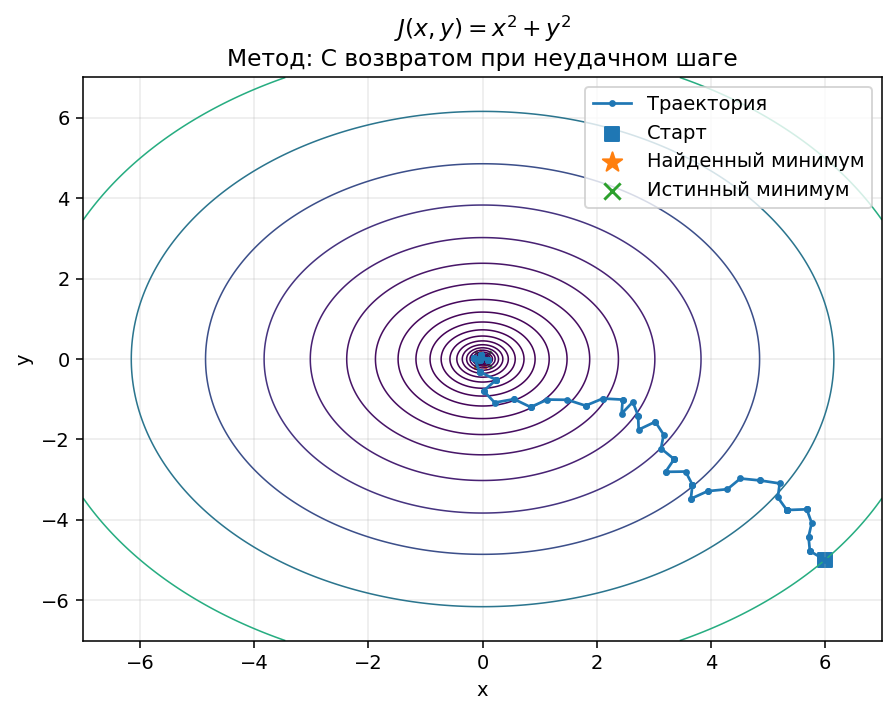
\includegraphics[width=0.82\textwidth]{graphs/f1_return.png}
\caption{С возвратом при неудачном шаге для функции f1.}
\end{figure}
\begin{figure}[H]
\centering
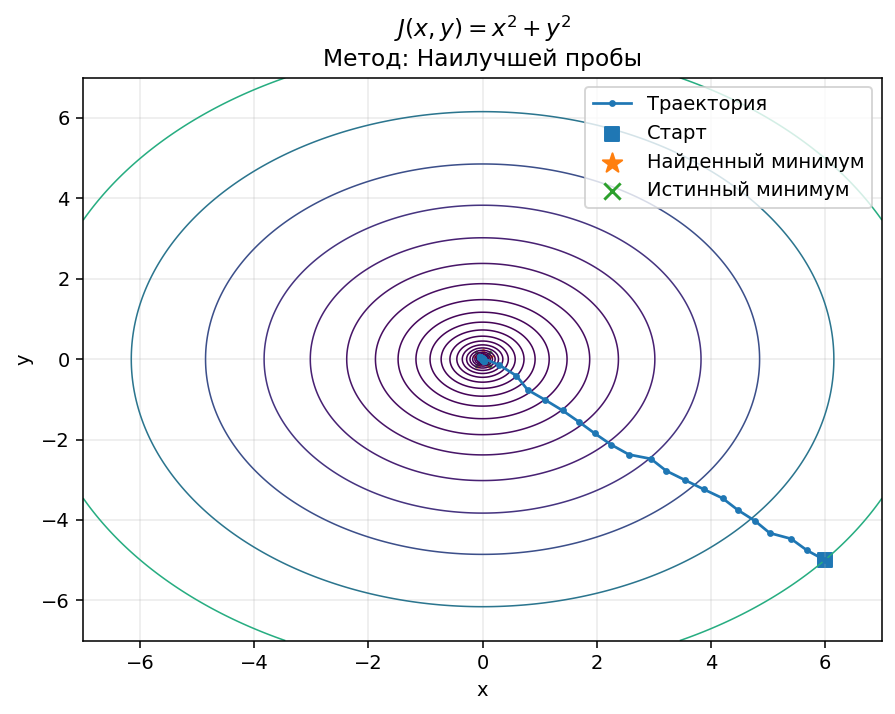
\includegraphics[width=0.82\textwidth]{graphs/f1_best_probe.png}
\caption{Наилучшей пробы для функции f1.}
\end{figure}
\begin{figure}[H]
\centering
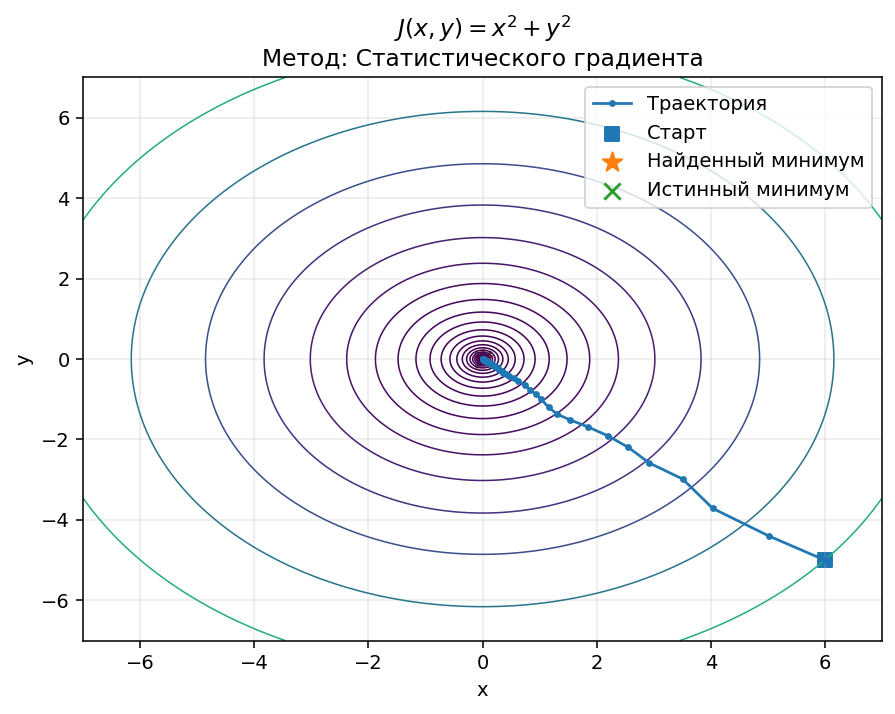
\includegraphics[width=0.82\textwidth]{graphs/f1_stat_grad.png}
\caption{Статистического градиента для функции f1.}
\end{figure}

\section{Функция f2: $J(x,y)=x^2/4+y^2/9$}
\begin{longtable}{|p{4.4cm}|p{2.4cm}|p{2.4cm}|p{2.8cm}|}
\hline
\textbf{Метод} & \textbf{$x_{\min}$} & \textbf{$y_{\min}$} & \textbf{$J(x_{\min}, y_{\min})$} \\ \hline
С возвратом при неудачном шаге & 0.000000 & 0.000000 & 0.000000 \\ \hline
Наилучшей пробы & 0.000000 & 0.000000 & 0.000000 \\ \hline
Статистического градиента & -0.000002 & 0.000000 & 0.000000 \\ \hline
\end{longtable}
\begin{figure}[H]
\centering
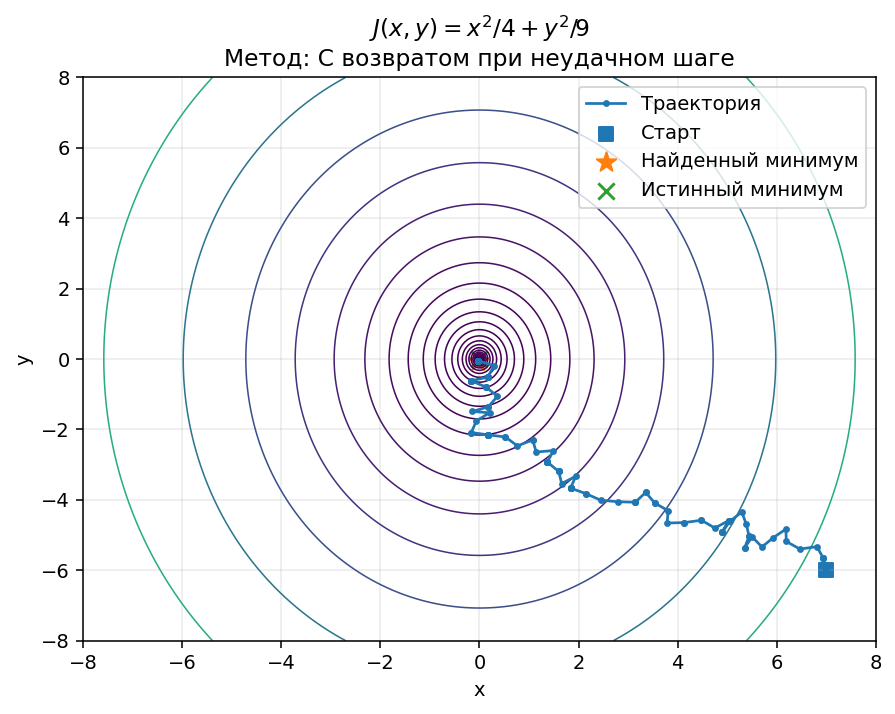
\includegraphics[width=0.82\textwidth]{graphs/f2_return.png}
\caption{С возвратом при неудачном шаге для функции f2.}
\end{figure}
\begin{figure}[H]
\centering
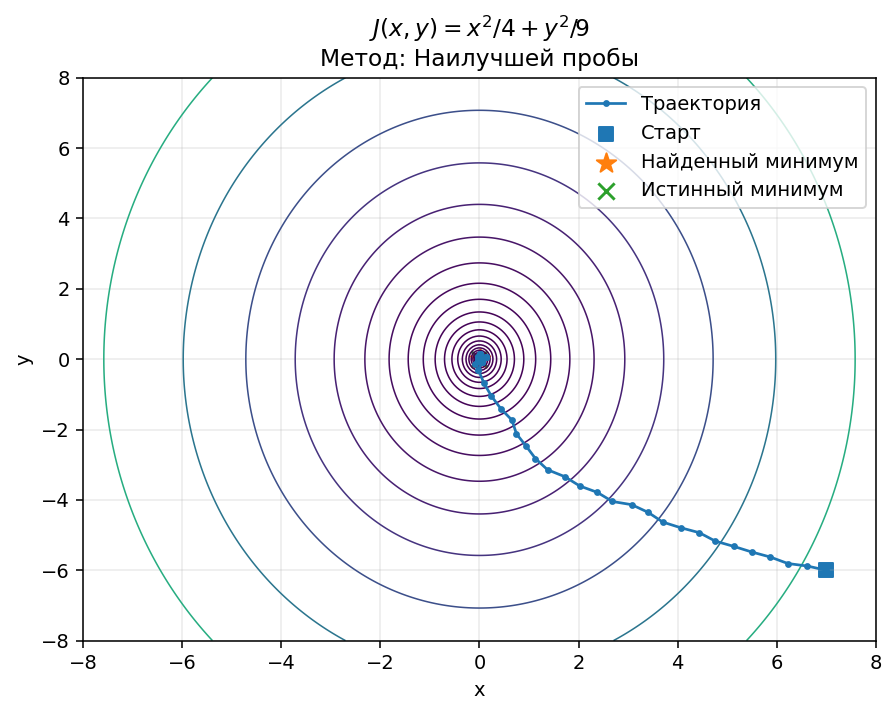
\includegraphics[width=0.82\textwidth]{graphs/f2_best_probe.png}
\caption{Наилучшей пробы для функции f2.}
\end{figure}
\begin{figure}[H]
\centering
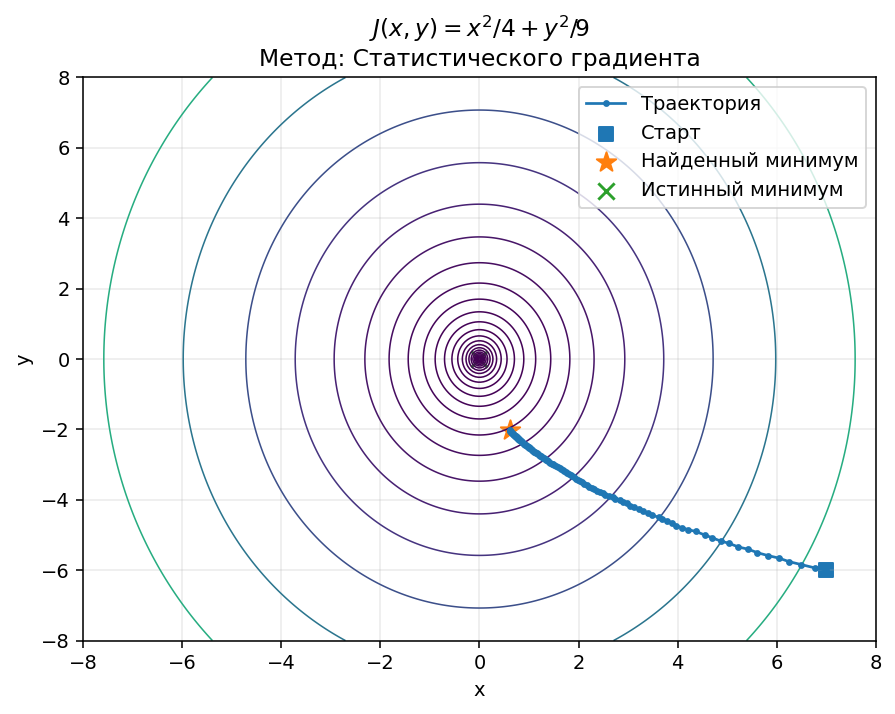
\includegraphics[width=0.82\textwidth]{graphs/f2_stat_grad.png}
\caption{Статистического градиента для функции f2.}
\end{figure}

\section{Функция f3: $J(x,y)=70(x-1)^2+(y-1)^2+1$}
\begin{longtable}{|p{4.4cm}|p{2.4cm}|p{2.4cm}|p{2.8cm}|}
\hline
\textbf{Метод} & \textbf{$x_{\min}$} & \textbf{$y_{\min}$} & \textbf{$J(x_{\min}, y_{\min})$} \\ \hline
С возвратом при неудачном шаге & 1.000000 & 0.999999 & 1.000000 \\ \hline
Наилучшей пробы & 1.000000 & 1.000000 & 1.000000 \\ \hline
Статистического градиента & 1.000000 & 1.000000 & 1.000000 \\ \hline
\end{longtable}
\begin{figure}[H]
\centering
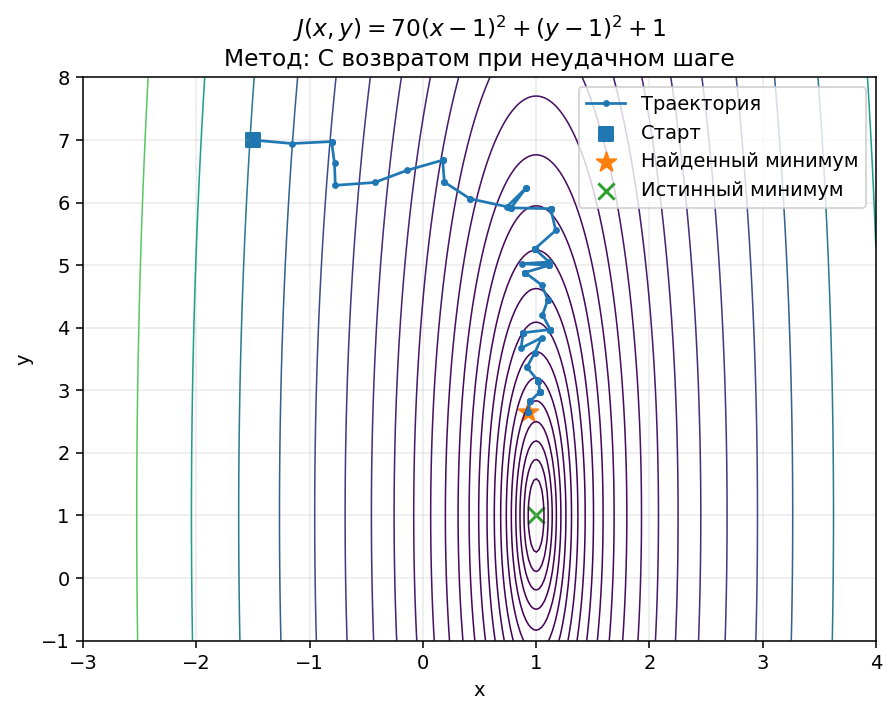
\includegraphics[width=0.82\textwidth]{graphs/f3_return.png}
\caption{С возвратом при неудачном шаге для функции f3.}
\end{figure}
\begin{figure}[H]
\centering
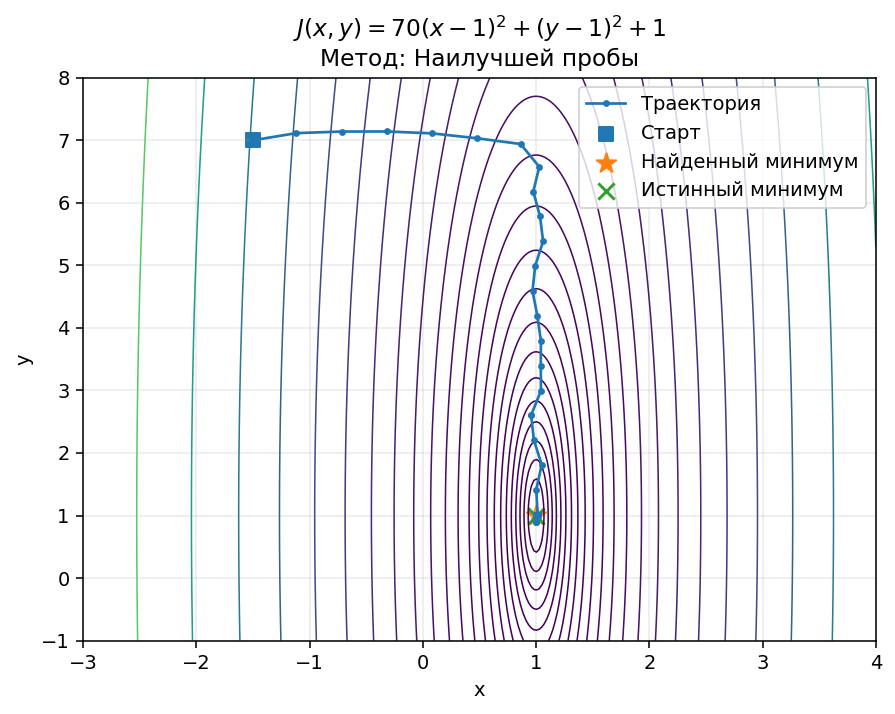
\includegraphics[width=0.82\textwidth]{graphs/f3_best_probe.png}
\caption{Наилучшей пробы для функции f3.}
\end{figure}
\begin{figure}[H]
\centering
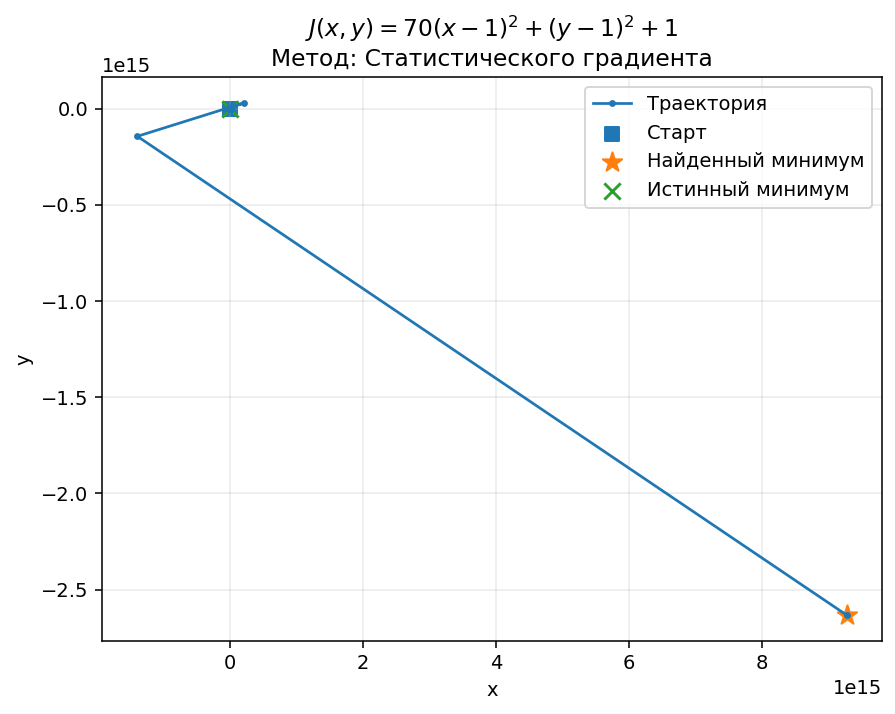
\includegraphics[width=0.82\textwidth]{graphs/f3_stat_grad.png}
\caption{Статистического градиента для функции f3.}
\end{figure}

\section{Функция f4: $J(x,y)=(x-8)^2+(y-1)^2+70(y+(x-8)^2-1)^2+1$}
\begin{longtable}{|p{4.4cm}|p{2.4cm}|p{2.4cm}|p{2.8cm}|}
\hline
\textbf{Метод} & \textbf{$x_{\min}$} & \textbf{$y_{\min}$} & \textbf{$J(x_{\min}, y_{\min})$} \\ \hline
С возвратом при неудачном шаге & 8.000000 & 1.000000 & 1.000000 \\ \hline
Наилучшей пробы & 8.000000 & 1.000000 & 1.000000 \\ \hline
Статистического градиента & 8.000000 & 1.000000 & 1.000000 \\ \hline
\end{longtable}
\begin{figure}[H]
\centering
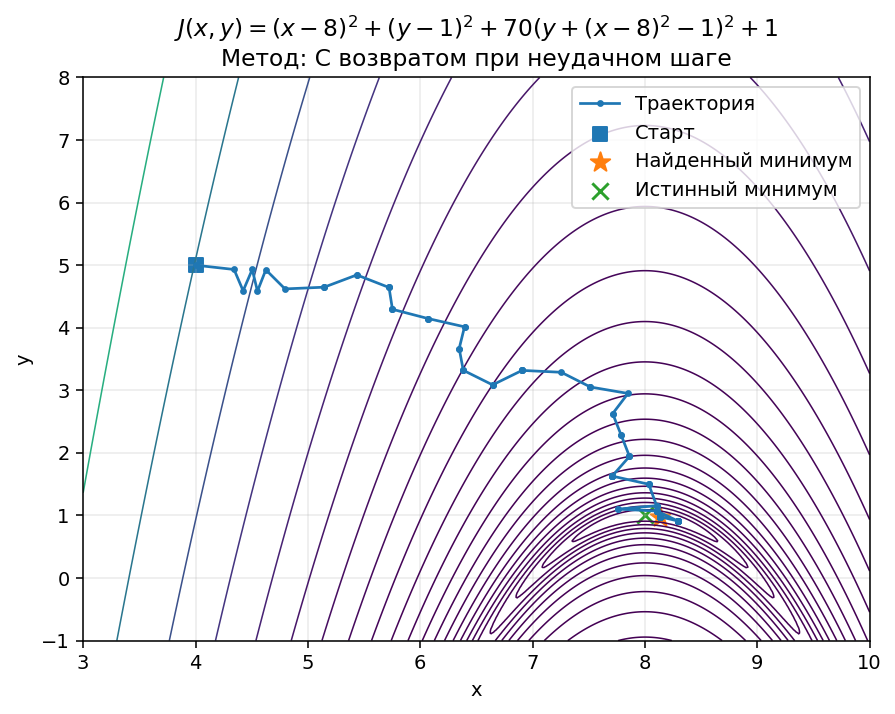
\includegraphics[width=0.82\textwidth]{graphs/f4_return.png}
\caption{С возвратом при неудачном шаге для функции f4.}
\end{figure}
\begin{figure}[H]
\centering
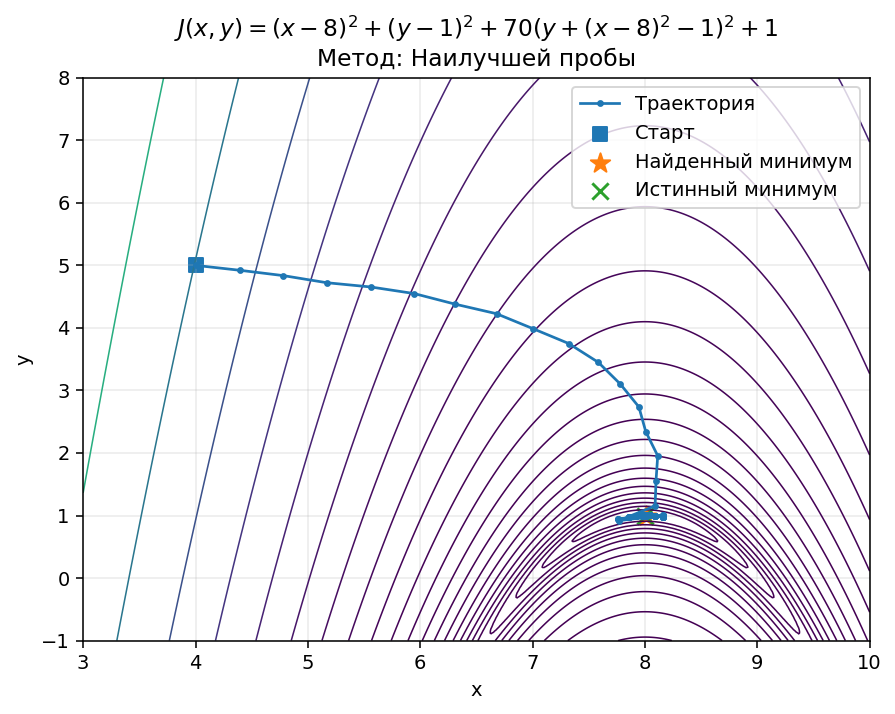
\includegraphics[width=0.82\textwidth]{graphs/f4_best_probe.png}
\caption{Наилучшей пробы для функции f4.}
\end{figure}
\begin{figure}[H]
\centering
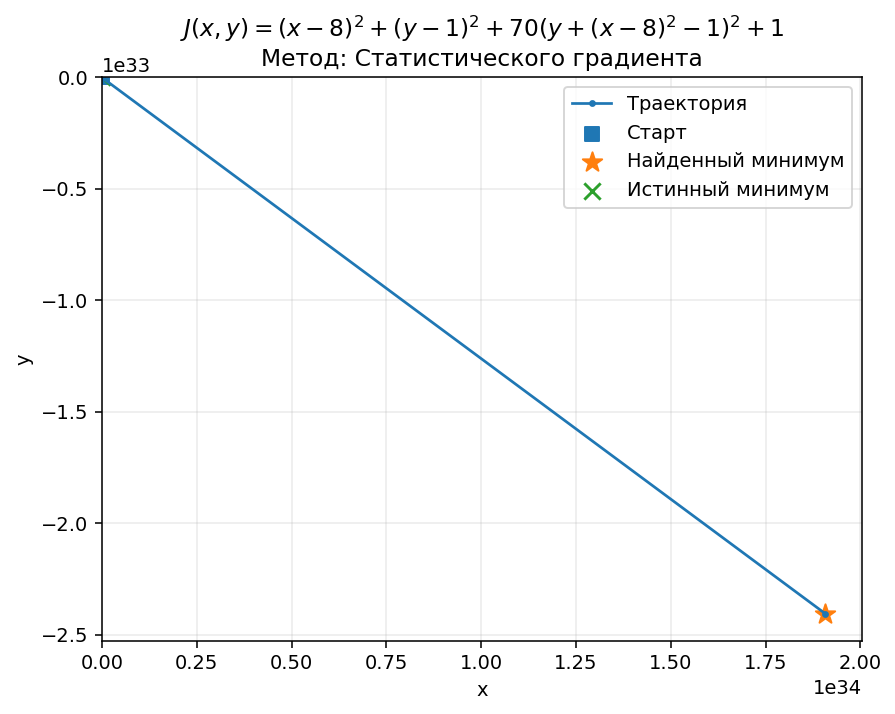
\includegraphics[width=0.82\textwidth]{graphs/f4_stat_grad.png}
\caption{Статистического градиента для функции f4.}
\end{figure}

\section*{Вывод}

Все три подхода позволяют приближаться к минимуму. Наиболее точные результаты на данных запусках даёт метод статистического градиента, особенно для гладких функций. Метод наилучшей пробы также показывает устойчивое поведение. Метод с возвратом при неудачном шаге работает проще, но обычно сходится медленнее и менее точно.

\end{document}
